\scanpage{3}

Chirurgie des surfaces conformes.

1) \uline{Découpage} : Découpe d'une surface conforme \deleted{\unsure{(sans bord|(avec bord}} (évt avec bord) suivant un sous-1-complexe rectifiable compact : On trouve une surface conforme à \deleted{\illegible{1}} bord, avec morceau \inserted{\deleted{compact}} de bord compact marqué.

2) \uline{Recollage} : À partir d'une surface conforme (avec bord \deleted{\unsure{à recoller|non vide}}) et d'un morceau compact de bord, et une relation d'équivalence ``admissible'' \inserted{(au sens rectifiable)} sur le bord, \deleted{\unsure{au sens}} on trouve une surface conforme avec bord...

3) \uline{Rétrécissage}
\[
\underset{\substack{\text{1-compl.}\\\text{cpt}}}{K}\subset
\underset{\text{s. conforme avec bord}}{X},
\]
$\widetilde X$ découpé de $X$ suivant $K$, $\partial'\widetilde X$ partie distinguée du bord, on choisit un \inserted{multi}anneau autour de $\partial'\widetilde X$, \deleted{soit alors} (un germe de tel anneau autour d'une composante $(\partial'_{\unsure{i}}\widetilde X)_i$ revient : la donnée d'une structure Riemannienne \deleted{\unsure{régulière}} \inserted{rectifiable} de long. totale 1 sur celle-ci....)

\figure{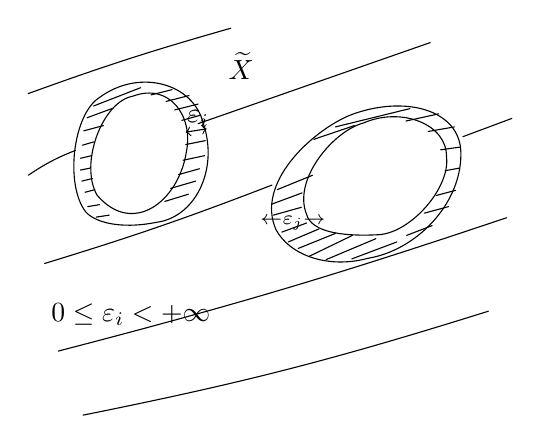
\begin{tikzpicture}[x=0.83cm,y=0.83cm,line cap=round,line join=round]
\draw[thin] (-0.6,2.5) to[bend left=2] (2.5,3.5);
\draw[thin] (-0.6,1.25) to[bend left=6] (0.12,1.63) (2.0,2.04) -- (5.55,3.28);
\draw[thin] (-0.35,-0.10) to[bend right=2] (3.13,1.10) (6.05,1.84) -- (6.80,2.12);
\draw[thin] (-0.14,-1.44) to[bend right=2] (6.72,0.60);
\draw[thin] (0.24,-2.42) to[bend right=3] (6.44,-0.83);
\draw (0.28,0.69) .. controls (-0.04,1.10) and (0.08,2.18) .. (0.49,2.44)
 .. controls (1.10,2.89) and (1.93,2.66) .. (2.08,2.04)
 .. controls (2.32,1.32) and (1.94,0.60) .. (1.36,0.53)
 .. controls (0.81,0.42) and (0.42,0.53) .. (0.28,0.69) -- cycle;
\draw (0.45,0.95) .. controls (0.18,1.44) and (0.54,2.38) .. (1.00,2.46)
 .. controls (1.56,2.67) and (1.93,2.16) .. (1.82,1.61)
 .. controls (1.70,0.84) and (0.99,0.31) .. (0.45,0.95) -- cycle;
\draw[thin] (0.40,2.31)--(1.12,2.59) (0.30,2.13)--(0.68,2.27) (0.25,1.93)--(0.55,2.01)
 (0.23,1.71)--(0.40,1.76) (0.20,1.51)--(0.37,1.55) (0.20,1.33)--(0.35,1.36)
 (0.22,1.16)--(0.38,1.20) (0.27,0.99)--(0.42,1.03) (0.31,0.77)--(0.49,0.80)
 (0.44,0.61)--(0.64,0.64) (1.28,2.48)--(1.60,2.56) (1.51,2.38)--(1.86,2.47)
 (1.64,2.25)--(2.00,2.34) (1.75,2.09)--(2.04,2.17) (1.81,1.72)--(2.11,1.78)
 (1.77,1.48)--(2.10,1.55) (1.70,1.26)--(2.02,1.35) (1.58,1.05)--(1.96,1.16)
 (1.49,0.85)--(1.85,0.96);
\draw[<->] (1.81,1.91)--(2.13,1.96);
\node[above,inner sep=0pt] at (2,1.98) {$\varepsilon_i$};
\node at (2.66,2.92) {$\widetilde X$};
\draw (3.19,0.42) .. controls (2.88,1.12) and (3.71,1.90) .. (4.30,2.16)
 .. controls (5.13,2.49) and (6.03,2.27) .. (6.02,1.57)
 .. controls (6.02,0.80) and (5.33,0.10) .. (4.60,-0.02)
 .. controls (3.97,-0.19) and (3.39,0.04) .. (3.19,0.42) -- cycle;
\draw (3.66,0.65) .. controls (3.44,1.18) and (4.07,1.93) .. (4.53,2.05)
 .. controls (5.10,2.30) and (5.81,2.04) .. (5.80,1.53)
 .. controls (5.86,1.06) and (5.25,0.36) .. (4.75,0.34)
 .. controls (4.14,0.31) and (3.73,0.40) .. (3.66,0.65) -- cycle;
\draw[thin] (3.21,1.03)--(3.75,1.25) (3.13,0.81)--(3.59,0.98) (3.15,0.64)--(3.58,0.76)
 (3.28,0.38)--(3.66,0.52) (3.38,0.23)--(3.85,0.43) (3.53,0.13)--(4.10,0.36)
 (3.70,0.01)--(4.36,0.33) (3.96,-0.04)--(4.72,0.28) (4.35,-0.03)--(5.04,0.23)
 (5.19,0.33)--(5.58,0.48) (5.46,0.67)--(5.83,0.77) (5.64,0.94)--(5.94,1.02)
 (5.78,1.32)--(6.00,1.36) (5.71,1.64)--(6.00,1.68) (5.52,1.92)--(5.92,1.99)
 (5.18,2.08)--(5.68,2.19) (4.10,1.99)--(5.24,2.27) (3.77,1.80)--(4.39,2.01);
\node[inner sep=0pt] at (3.45,0.52) {$\scriptstyle\leftarrow\varepsilon_j\rightarrow$};
\node at (0.97,-0.88) {$0\leq\varepsilon_i<+\infty$};
\end{tikzpicture}}

$\widetilde X^*$ la surface \inserted{à bord \deleted{\unsure{décrit}} \deleted{\unsure{défini}} \unsure{dite}} rétrécie déduite de la connue choisissons un isomorphisme rectifiable $\partial'\widetilde X^*\xrightarrow{\sim}\partial'\widetilde X$ compatible avec les comp. connexes, et utilisons la relation d'équivalence \inserted{de \unsure{recollement|recollage}} sur $\partial'\widetilde X$ pour en déduire une sur $\widetilde X^*$. On en conclut \deleted{$\unsure{K}$} $X^*$ et $K\subset X^*$

% archive sheet number: 2
